\Chapter{Introduction}
\label{Introduction}
	\section{Fondamentaux de la physique des plasmas}
		 
\emph{Le plasma}. Le plasma est souvent considéré un peu équivoquement comme le
quatrième état de la matière. Dans notre environnement proche, nous avons pris
conscience de son existence à travers les phénomènes de flammes, d'éclairs,
d'aurore boréales ou d'arc électriques. Mais à des conditions de pressions et de
températures différentes de celles de notre atmosphère terrestre, il est
omniprésent : plus de 99\% de la matière connue est sous cette forme.
		
Une définition plus adaptée du plasma est celle d'un gaz conducteur. Une partie
des atomes le composant est ionisée, donnant naissance à une population
d'électrons libres et d'ions de différentes espèces. Ces populations permettent
alors le transport de courant et, sensibles aux forces électromagnétiques,
influencent fortement le comportement global du plasma en provoquant des
phénomènes collectifs, non-linéaires et turbulents.
		
Le plasma et son comportement sont décrits par la théorie de la physique des
plasmas. Elle intègre les connaissances de nombreux domaines, tels que la
physique statitique, l'électromagnétisme, ou encore la dynamique des fluides.
		
		\subsection{Les paramètres plasmas}
		
Les plasmas se définissent donc comme des gaz possédant une population
d'électrons libres $n_e$ à une température électronique $T_e$.
La figure \ref{zoologie}, issue du livre du National Research
Council\cite{national1995Plasma}, représente une classification des plasmas en
fonction de ces deux paramètres principaux qui vont influer sur la dynamique du
transport de courant.
La théorie présentée dans la suite de cette thèse ne concerne que les plasmas
dits classiques :
			\begin{itemize}
			  \item les plasmas naturels peu dense tels que l'espace interstellaire,
			  le vent solaire, la magnétosphère, et l'ionosphère
			  \item les plasmas naturels denses tels que les éclairs et les étoiles
			  \item les plasmas industriels, de laboratoire, et thermonucléaires
			\end{itemize}
			\begin{figure}[htbp]
				\centering
				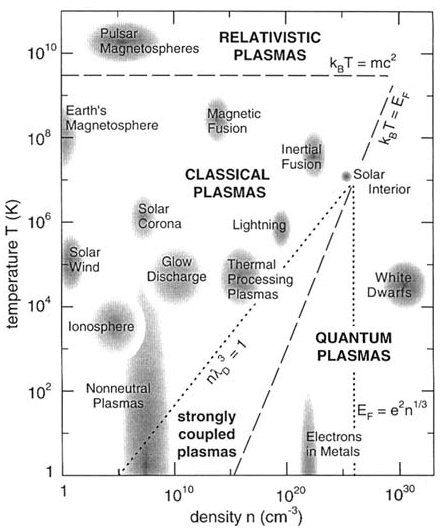
\includegraphics[height=80mm,width=64mm]{figures/zoologie.png}{\caption{Classification
				de différents plasmas en fonction de $n_e$ et $T_e$.}\label{zoologie}}
			\end{figure}
			
			Dans ces plasmas, le dégré d'ionisation $\alpha$ est donné par le rapport
			entre la densité électronique $n_e$ et la densité de gaz $n_g$ :
			\begin{equation}
				\alpha=\frac{n_e}{n_e+n_g}
			\end{equation}
			Cette fraction va définir l'importance de l'interaction entre les particules 
			neutres et les particules chargées. Cependant, même à très faible $\alpha$,
			l'apparition d'une population de porteurs de charge va modifier les caractéristiques et la
			dynamique du plasma. 
			
			L'ionisation du gaz suit l'évolution de la température électronique $T_e$ qui
			mesure l'agitation thermique des électrons. Densité et température
			électronique permettent de définir le paramètre plasma:
			\begin{equation}
				\Gamma=\frac{<E_p>}{<E_c>}=\frac{e^2n_e^{1/3}}{\varepsilon_{_0} eT_e}
			\end{equation}
			Le paramètre plasma représente le ratio entre l'énergie thermique des
			électrons et leur énergie potentielle électrostatique coulombienne \emph{ie.}
			l'agitation thermique desordonnée contre les forces d'interactions
			coulombiennes structurantes. 
			
			Les plasmas classiques (ou cinétiques) sont caractérisés par
			$\Gamma\ll 1$. Ils ont une population d'électrons assez espacée et/ou une
			température suffisamment élevée.
			
		\subsection{Echelles et phénomènes collectifs}
		La dynamique d'un plasma résulte du couplage entre le mouvement des
		particules chargées et les forces électromagnétiques $\mathbf
		F=q_s\mathbf + q_s\mathbf v_s\times\mathbf B$)
		présentent ou qui se forment dans le système.
		Elle peut se décomposer sur deux échelles de temps qui correspondent à l'équilibre électrostatique
		et à l'équilibre thermodynamique.
		\subsection{Quasineutralité}
			Le processus le plus rapide est lié à
			l'équilibre microscopique électrostatique qui s'opère lors de la formation
			d'un plasma entre l'agitation thermique et l'interaction coulombienne. Les
			ions et des électrons issus de l'ionisation se réorganisent pour écranter
			leur champ électrique individuel et former ainsi un ensemble électriquement neutre. 
			Ce comportement est décrit aux plus petites échelles spatiotemporelles par
			le principe fondamental de la dynamique et la loi de Boltzman-Poisson :
			\begin{align}
				m_s\frac{\partial \mathbf{v}}{\partial t}=q_s\mathbf E
				\;\;\;\;\;\;\text{et}\;\;\;\;\;\;
				\nabla^2\Phi=\frac{\rho}{\varepsilon_{_0}}
			\end{align} 
			où $m_s$ est la masse de la particule, $\mathbf{v}$ sa vitesse, $q_s$ la
			charge élémentaire, $\rho$ la densité de charge, résultant de la différence entre la 
			densité ionique et la densité électronique.
			Les échelles fondamentales entrant en jeu sont alors la pulsation plasma et
			la longueur de Debye, reliée à la vitesse thermique 
			\begin{equation}
				\omega_p=\sqrt{\frac{n_{_0}e^2}{\varepsilon_{_0}
				m_e}}\;\text{,}\;\;\;\lambda_D=\sqrt{\frac{\varepsilon_{_0}
				eT_e}{n_{_0}e^2}}\;\;\;\text{et}\;\;\;v_{th}=\sqrt{\frac{eT_e}{m_e}}
			\end{equation}
			Au dela de ces échelles, on peut considérer cette dynamique comme instantanée
			et uniforme. Globalement, vu de suffisement loin et exepté à ses frontières,
			le plasma est dans un état de \emph{quasi-neutralité}, \emph{ie.} $n_e=n_i$.
			
			Une fois cet équilibre mis en place, le système évolue par le biais de
			\emph{phénomènes de transport} résultants de la tendance à
			l'homogénéisation du plasma par collisions entres les particules et de
			l'influence globale des champs électromagnétiques. On parle notamment de
			processus de diffusion/convection de particules, de viscosité (transfert de
			quantité de mouvement), de conductivité (transport de charges) ou encore de
			conductivité thermique (transport de chaleur). Dans les plasmas
			classiques, ces phénomènes interviennent sur des échelles relativements
			lentes et relativement grandes devant $\omega_p$ et $\lambda_D$.
		\subsection{Collisions}
			Dans un plasma, les collisions représentent les interactions binaires
			directes entre électrons, ions et atomes neutres. Elles sont
			définies pour chaque couple d'espèces de particules et catégorisées suivant
			leur nature élastique ou inélastique, entraînant pour chacun des cas des
			comportements spécifiques.
			
			\textbf{Collisions élastiques}
			
		\subsection{Plasma et champ magnétique}
			%\begin{wrapfigure}{r}{0.50\textwidth}
    		%	\vspace{-5pt}
    		%
    		%	%
    		%	%
    			% \hspace{20pt}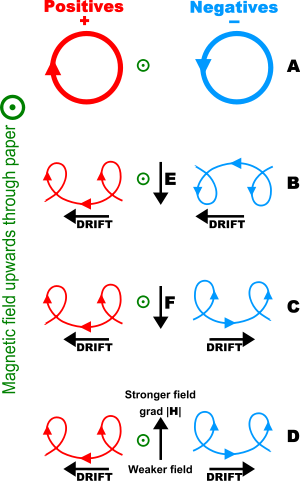
\includegraphics[width=0.40\textwidth]{figures/particleDrifts.png} \hspace{20pt}\caption{Mouvement cyclotronique et de dérive des particules
    		%	dans un champ magnétique.}\label{particleDrifts}
  			%	 \vspace{-20pt}
			%\end{wrapfigure}
			\begin{figure}
				\centering
				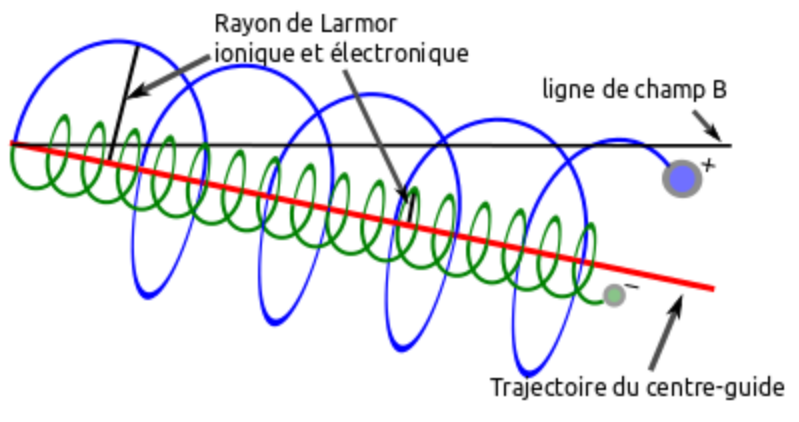
\includegraphics[width=0.8\textwidth]{figures/mouvementCyclotron.png}
				{\caption{Mouvement cyclotronique des particules autour des lignes de champ
				magnétique.}\label{1-particleDrifts}}
			\end{figure}
			La présence d'un champ magnétique influence aussi fortement le transport global qui 
			se met en place dans les plasmas. Sous l'action de la force de Lorentz, les particules 
			chargées sont en rotation autour des lignes de champ magnétique. En l'absence de force 
			extérieure, les particules sont confinéesLeur mouvement peut alors
			se décrire par trois composantes (cf. figure \ref{1-particleDrifts}) :			
			\begin{itemize}
			\item Un déplacement parallèle aux lignes de champ, de l'ordre de la vitesse
			thermique de l'espèce, $v_\para\approx c_s=(eT_s/m_s)^{\text{\textonehalf}}$
			\item Le mouvement cyclotronique, rotation rapide de la particule
			autour des lignes de champ magnétiquedans le plan perpendiculaire aux lignes
			de champ
			\item Une vitesse de dérive, 
			\end{itemize}
			\
			
			
			
			Dans suite de cette thèse, nous allons étudier la dynamique électrique d'un plasma en milieu magnétisé
			, ie. ou les 
			des structure et de la dynamique essentiellement reliée aux variations du champ électrique.
	\section{Description fluide d'un plasma}
		
		\subsection{De la statistique au fluide}
			$$\partial_tf_s+\mathbf{v}_s\cdot\vec\nabla_\mathbf{r}f_s+\frac{\mathbf{F}_s}{m_s}\cdot\vec\nabla_{\mathbf{v}_s}f_s=\partial_tf_{|_{coll}}$$
			Braginskii equations
			$$M^{(k)}_s=\int_{-\infty}^{\infty}\mathbf{v}_s^kf_sd\mathbf{v}$$
		\subsection{Conservation de la matière}
			$$n_s=\int f_sd\mathbf{v}$$
			
		\subsection{Conservation de l'impulsion}
			$$n_s\mathbf{v}_s=\int \mathbf{v}_sf_sd\mathbf{v}$$
		\subsection{Conservation de l'énergie}
		\subsection{Conservation de la chaleur}
	\section{Les gaines électrostatiques}
			Les gaines électrostatiques sont des structures non-neutres qui se
			développent à la frontière entre un plasma et un objet. Elles apparaissent
			spontanément du fait de la plus grande vitesse des électrons par rapport à
			celle des ions. D'une taille de l'ordre de quelques longueurs de Debye $\lambda_D$, 
			L'interaction dite plasma-paroi est une branche à part entière de la physique des plasmas.
			En effet, au contact d'un milieu extérieur, que ce soit un obstacle matériel
			ou un gaz ambiant, le plasma perd sa quasineutralité.
			\subsection{Physique de la prégaine}
			\subsection{Physique de la gaine}
			\subsection{Gaine dans les plasmas magnétisés}
			\subsection{Problématique de la gaine parallèle aux lignes de champ}
	
	 \section{Les décharges plasma basse-pression}
		\subsection{Création de la décharge, rôle des électrons}
		Dans les plasmas basse-température industriels et de laboratoires, qui possédent
			un faible degré d'ionisation, ou dans l'ionospère, la dynamique du plasma est dominée par
			la perte de quantité de mouvement dûe à l'ionisation la force de friction avec le gaz.
		Electrical breakdown, Townsend avalanche, 
		\subsection{Trasport des ions et champ ambipolaire}
		\begin{equation}
			\label{derivediffusion}
		\end{equation}
		\subsection{Equations de dérive-diffusion magnétisées}
		
	\section{Les plasmas de bord des tokamaks}
		Lawson criteriom, strongly magnetized
		\subsection{La fusion et les tokamaks}
		\subsection{Le plasma de la Scrape-of-Layer}
		\subsection{Les vitesses de dérives}
		\label{vitessesDerive}
	\section{Les modèles numériques}
		L'étude de phénomènes complexes
		%\begin{figure}[htbp]
		%	\centering
		%	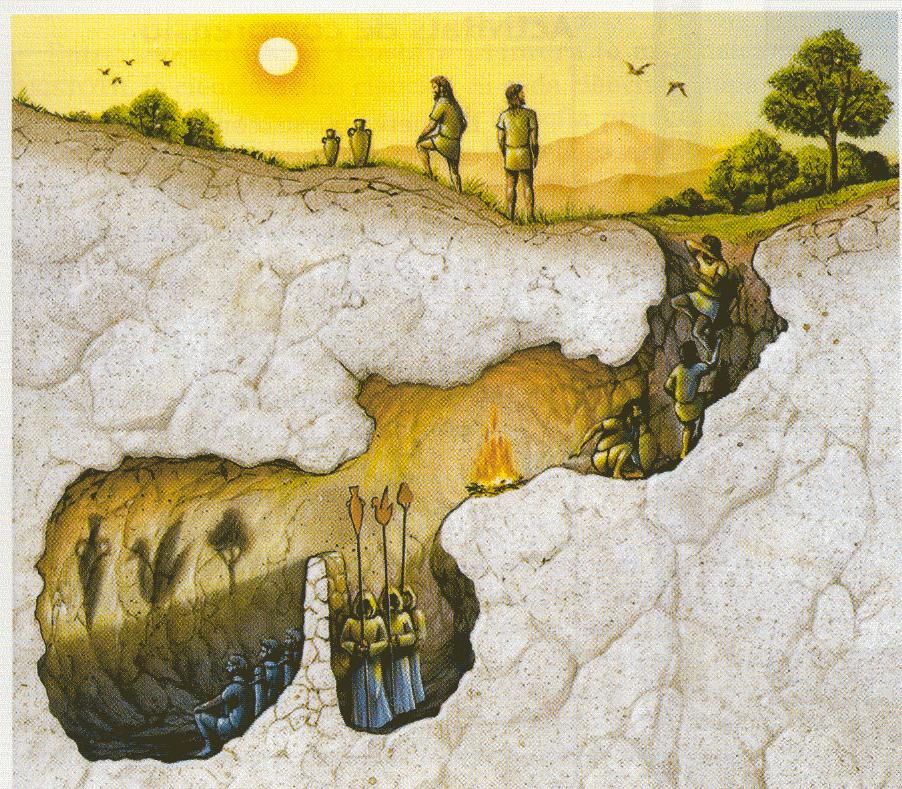
\includegraphics[height=64mm]{figures/cave.jpg}
		%	{\caption{La caverne des idées.}\label{caverne}}
		%\end{figure}
		%\begin{figure}[htbp]
%
%			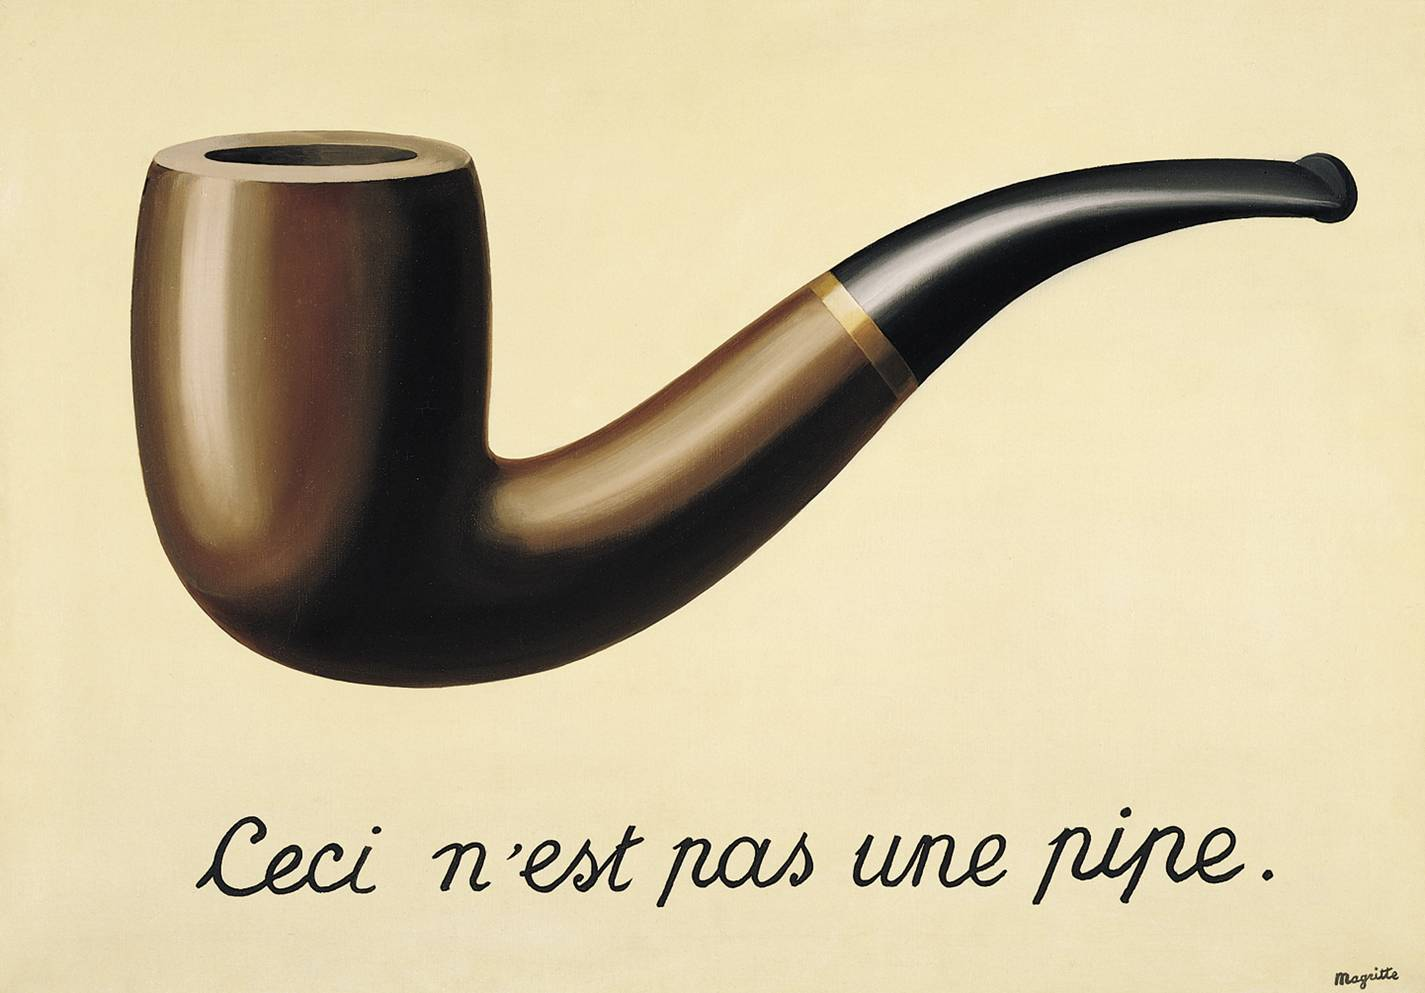
\includegraphics[height=40mm]{figures/Magritte.jpg}
%			{\caption{Magritte. La trahison des images.}\label{magritte}}
%		\end{figure}


	
	

		